\documentclass[aspectratio=169]{beamer} % O parâmetro aspectratio com valar 16:9 deixa o slide em widescreen

\usepackage[brazil]{babel}
\usepackage[utf8]{inputenc}
\usepackage[T1]{fontenc}

\usetheme{Madrid}
\setbeamertemplate{navigation symbols}{}

\title[Informática]{Informática}

\author[Diego S. C. Nascimento]{Diego Silveira Costa Nascimento}

\institute[IFRN]{
Instituto Federal de Educação, Ciência e Tecnologia do Rio Grande do Norte\\
diego.nascimento@ifrn.edu.br
}

\date[\today]{\today}

\begin{document}

\begin{frame}[plain]
	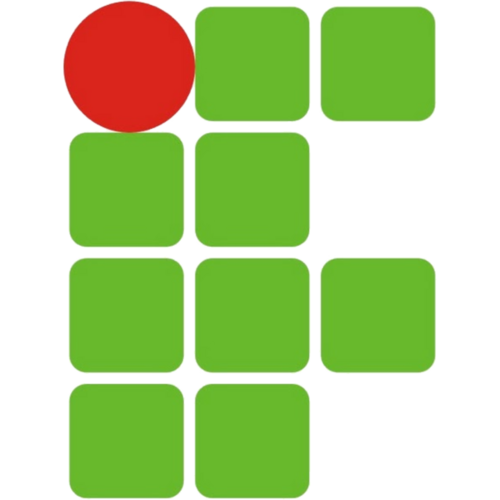
\includegraphics[scale=0.2]{img/IFRN}
	\titlepage
\end{frame}

\logo{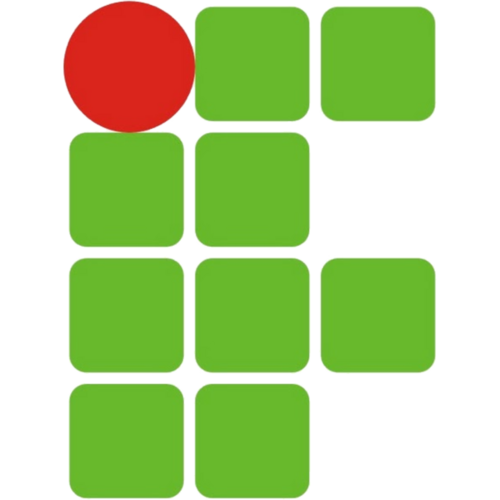
\includegraphics[scale=0.1]{img/IFRN}}

\begin{frame}
	\frametitle{Ementa do Curso}
  	\tableofcontents
\end{frame}

\AtBeginSection[]{
	\begin{frame}
		\frametitle{Ementa}
		\tableofcontents[currentsection]
	\end{frame}
}

\section{Introdução}

\begin{frame}
	\frametitle{História}
	
	\begin{itemize}
		\item Parte da evolução aconteceu ao mero acaso;
		\item A outra parte se deve a poucos homens que observaram os problemas cotidianos e tentaram encontrar um solução;
		\item Cada época apresentada seus principais pensadores, inventores e pessoas de diversos níveis de conhecimento;
		\item Para que uma invenção pudesse ser conhecida, havia uma demora de anos ou décadas; e
		\item O intervalo de conhecimento e de descobertas da humanidade vai diminuindo consideravelmente.
	\end{itemize}
\end{frame}

\begin{frame}
	\frametitle{As mãos}
	
	\begin{itemize}
		\item Primeira forma de mostrar uma quantidade; 
		\item Serviram como instrumentos de comparação; e
		\item Provavelmente aí está a origem do nosso sistema de numeração de base decimal (10 dedos).
	\end{itemize}\vfill
	
	\begin{exampleblock}{Ilustra\c cão}
	\end{exampleblock}
\end{frame}

\begin{frame}
	\frametitle{Pastor de ovelhas}
	
	\begin{itemize}
		\item Primeiro ser humano a calcular;
		\item Em latim, pedrinha se escreve \textit{calculu}.
	\end{itemize}\vfill
	
	\begin{exampleblock}{Ilustra\c cão}
	\end{exampleblock}
\end{frame}

\begin{frame}
	\frametitle{Ábaco}
	
	\begin{itemize}
		\item Provavelmente inventado na China (Dinastia de Yuan); e
		\item É o primeiro instrumento de calcular que se tem conhecimento.
	\end{itemize}\vfill
	
	\begin{exampleblock}{Ilustra\c cão}
	\end{exampleblock}
\end{frame}

\begin{frame}
	\frametitle{Ossos de Napier}
	
	\begin{itemize}
		\item John Napier foi um matemático escocês;
		\item Desenvolveu um conjunto de noves bastões chamados de Ossos de Napier; e
		\item Eram usados para multiplicar e dividir números elevados.
	\end{itemize}\vfill
	
	\begin{exampleblock}{Ilustra\c cão}
	\end{exampleblock}
\end{frame}

\begin{frame}
	\frametitle{Pascalina}
	
	\begin{itemize}
		\item Blaise Pascal, em 1642, inventou a primeira máquina de somar;
		\item Executava operações aritméticas quando se giravam os discos interligados; e
		\item Foi a precursora das calculadoras mecânicas.
	\end{itemize}\vfill
	
	\begin{exampleblock}{Ilustra\c cão}
	\end{exampleblock}
\end{frame}

\begin{frame}
	\frametitle{Máquina de Leibnitz}
	
	\begin{itemize}
		\item O alemão Gottfried Wilhelm Leibnitz, em 1671, inventou uma máquina muito parecida com a Pascalina;
		\item Efetuava cálculos de multiplicação e divisão; e
		\item Se tornou a antecessora direta das calculadoras manuais.
	\end{itemize}\vfill
	
	\begin{exampleblock}{Ilustra\c cão}
	\end{exampleblock}
\end{frame}

\begin{frame}
	\frametitle{Máquina de Leibnitz}
	
	\begin{itemize}
		\item O alemão Gottfried Wilhelm Leibnitz, em 1671, inventou uma máquina muito parecida com a Pascalina;
		\item Efetuava cálculos de multiplicação e divisão; e
		\item Se tornou a antecessora direta das calculadoras manuais.
	\end{itemize}\vfill
	
	\begin{exampleblock}{Ilustra\c cão}
	\end{exampleblock}
\end{frame}

\begin{frame}
	\frametitle{Tear mecânico de Jacquard}
	
	\begin{itemize}
		\item Joseph-Marie Jacquard, em 1801, inventou um tear mecânico;
		\item Utilizava cartões perfurados;
		\item Fazia combinações de desenhos mais sofisticadas; e
		\item Cartões perfurados seriam posteriormente usados para projetar máquinas de calcular.
	\end{itemize}\vfill
	
	\begin{exampleblock}{Ilustra\c cão}
	\end{exampleblock}
\end{frame}

\begin{frame}
	\frametitle{Máquina diferencial}
	
	\begin{itemize}
		\item Charles Babbage é conhecido como o \structure{Pai da Computação};
		\item Em 1822, desenvolveu a máquina diferencial de Babbage; 
		\item Permitia cálculos de funções trigonométricas e logarítmicas; e 
		\item Utilizava os cartões de Jacquard.
	\end{itemize}\vfill
	
	\begin{exampleblock}{Ilustra\c cão}
	\end{exampleblock}
\end{frame}

\begin{frame}
	\frametitle{Máquina analítica}
	
	\begin{itemize}
		\item Charles Babbage, em 1834, desenvolveu a máquina analítica;
		\item Permitia somar, dividir, subtrair e multiplicar;
		\item Armazenava dados em memória de até 1000 números de 50 dígitos; e 
		\item Imprimia resultados;
	\end{itemize}\vfill
	
	\begin{exampleblock}{Ilustra\c cão}
	\end{exampleblock}
\end{frame}


\end{document}